\documentclass[a4paper]{article}

\usepackage{graphicx}
\usepackage{float}
\usepackage{hyperref}
\usepackage{xcolor}
\usepackage[spanish]{babel}
\usepackage{listings}
\usepackage{enumitem}
\usepackage[utf8]{inputenc}

\lstset{language=c, frame=tlrb, basicstyle=\scriptsize, breaklines=true, numberbychapter=false,numbers=left}
\setlist[enumerate]{noitemsep}
\setlist[itemize]{noitemsep}

\begin{document}

\title{Infraestructura de Análisis de Rendimiento\\
\bigskip
{\large Propuesta de tesis para\\} Magister en Cómputo de Altas Prestaciones\\
\bigskip
Universidad Nacional de La Plata\\
Facultad de Informática\\
\bigskip
}

\author{Tesista: Andrés More - {\tt amore@hal.famaf.unc.edu.ar}\\
Director: Dr. Fernando G. Tinetti - {\tt fernando@lidi.info.unlp.edu.ar}}

\date{Octubre de 2013}

\maketitle

\newpage

\section{Objetivo}

La propuesta principal consiste en el desarrollo de una infraestructura de soporte para el análisis de aplicaciones de Cómputo de Altas Prestaciones.

\smallskip

Como se demuestra en la Figura \ref{fig:framework}, la infraestructura implementa una serie de etapas donde se automatiza un proceso de análisis de rendimiento ejecutando pruebas de referencia, herramientas de perfil de rendimiento, análisis de resultados y compilación de un reporte.

\begin{figure}[H]
\centering
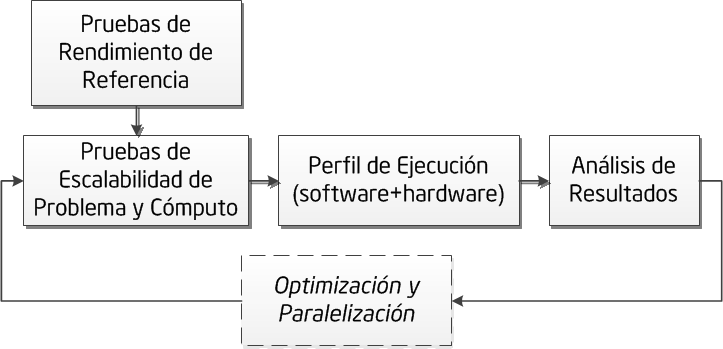
\includegraphics{framework.png}
\caption{Infrastructura a Desarrollar}
\label{fig:framework}
\end{figure}

\section{Motivación/Estado del Arte del Tema}

Expertos de dominio no son expertos en análisis de rendimiento.

\smallskip

Continuación del trabajo final de la especialización.

\section{Temas de Investigación}

Esta sección contiene una lista inicial de los temas a desarrollar.

\begin{enumerate}
\item Análisis automático de rendimiento
\end{enumerate}

\section{Desarrollos/Trabajo Experimental a Realizar}

La infraestructura a desarrollar consiste de distintos componentes:

  \begin{enumerate}
  \item Componente de ejecución de pruebas de rendimiento.
  \item Componente de aplicación de herramientas de soporte.
  \item Componente de análisis de datos de rendimiento.
  \item Componente de reporte de rendimiento.
  \end{enumerate}

% chart?
% hidef model?

% Execution (Figures) / Analysis (Laws) / Reporting (PDF)

\section{Esquema de Plan de Trabajo}

El siguiente cronograma muestra el plan de actividades tentativo incluyendo actividades y tiempos.
Es de notar que el trabajo es una continuación de un trabajo final de especialización.

\begin{table}[H]
    \caption{Detalle de Actividades}
  \centering
    \begin{tabular}{|l|l|}\hline
      {\bf Actividad} & {\bf Duración} \\ \hline
      Diseño de Alto Nivel & Noviembre \\ \hline
      Prototipo & Diciembre-Enero \\ \hline
      Pruebas de Rendimiento & Febrero \\ \hline
      Calculo de Leyes & Marzo \\ \hline
      Perfil de Rendimiento & Abril \\ \hline
      Eventos y Vectorización & Mayo-Junio \\ \hline
    \end{tabular}
  \label{schedule}
\end{table}

\section{Posibilidades de Realización}

El alumno tiene a su disposición acceso al equipamiento necesario como parte de su ámbito laboral.
El alumno trabaja como Ingeniero en Software en Argentina Software Design Center (ASDC - Intel Córdoba); también
como docente e investigador en el Instituto Universitario Aeronáutico dictando tanto cursos de grado (Cómputo de Altas Prestaciones) como postgrado (Implementación de Sistemas Operativos).

\section{Bibliografía Básica Relacionada}

Un conjunto inicial a modo de referencia es incluido en la bibliografía listada a continuación.

\begin{thebibliography}{9}
  
\bibitem{critical-overview}
 J. Browne,
 \emph{A critical overview of computer performance evaluation},
 1976.

\bibitem{patterns}
 G. Mattson, B.A. Sanders and B.L. Massingill, 
 \emph{Patterns for Parallel Programming, Addison-Wesley},
 2004.

\bibitem{automatic-performance-analysis}
 T. Margalef, J. Jorba, O. Morajko, A. Morajko, E. Luque,
 \emph{Different approaches to automatic performance analysis of distributed applications},
 2004.

\bibitem{intro-software-performance}
 C. Smith,
 \emph{Introduction to software performance engineering: origins and outstanding problems},
 2007.

\bibitem{future-software-performance}
 M. Woodside, G. Franks, D. Petriu,
 \emph{The Future of Software Performance Engineering},
 2007.

\bibitem{capturing-performance-knowledge}
 K. Huck, O. Hernandez, V. Bui, S. Chandrasekaran, B. Chapman, A. Malony, L McInnes, B. Norris,
 \emph{Capturing performance knowledge for automated analysis},
 2008.

\bibitem{spec}
  Andres More,
 \emph{Herramientas de Soporte para Análisis de Rendimiento},
 Trabajo Final Especializacion HPC/GRID - UNLP 2013.

\bibitem{counters}
  Fernando G. Tinetti, Mariano Mendez, and Armando De Giusti,
  \emph{An Automated Approach to Hardware Performance Monitoring Counters},
  2013. 

% http://en.wikipedia.org/wiki/Performance_tuning

\end{thebibliography}

\end{document}
